% Comprehensive TikZ Diagrams for VerletDrift Mathematical Equations
% These diagrams can be included in the main sections with % Comprehensive TikZ Diagrams for VerletDrift Mathematical Equations
% These diagrams can be included in the main sections with % Comprehensive TikZ Diagrams for VerletDrift Mathematical Equations
% These diagrams can be included in the main sections with % Comprehensive TikZ Diagrams for VerletDrift Mathematical Equations
% These diagrams can be included in the main sections with \input{diagrams.tex}
% or individual diagrams can be copy-pasted where needed.

% ==============================================================================
% DIAGRAM 1: CAR BODY GEOMETRY
% ==============================================================================
% Use in Section 1 (Verlet Integration) to show car structure

\begin{figure}[h]
  \centering
  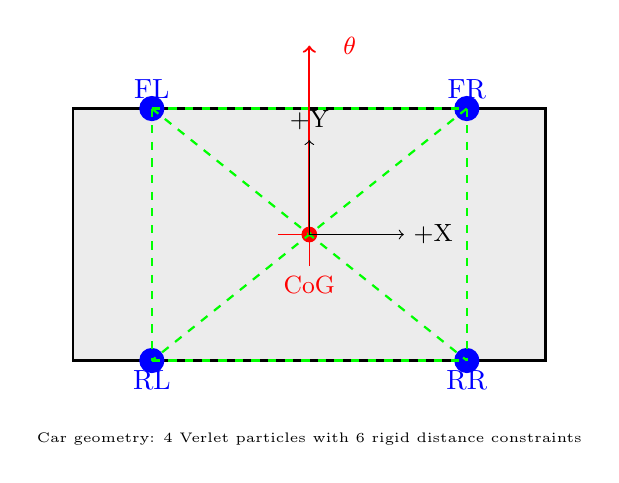
\begin{tikzpicture}[scale=2, thick]
    % Car body (rectangle)
    \draw[fill=lightgray!30] (-1.5, -0.8) rectangle (1.5, 0.8);
    \draw (-1.5, -0.8) -- (1.5, -0.8) -- (1.5, 0.8) -- (-1.5, 0.8) -- cycle;

    % Center of mass (crosshair)
    \fill[red] (0, 0) circle (0.05);
    \draw[red, thin] (-0.2, 0) -- (0.2, 0);
    \draw[red, thin] (0, -0.2) -- (0, 0.2);
    \node[red, below, font=\small] at (0, -0.2) {CoG};

    % Wheel positions (Verlet particles)
    \fill[blue] (-1.0, -0.8) circle (0.08);
    \fill[blue] (1.0, -0.8) circle (0.08);
    \fill[blue] (-1.0, 0.8) circle (0.08);
    \fill[blue] (1.0, 0.8) circle (0.08);

    % Labels
    \node[blue, above] at (-1.0, 0.8) {FL};
    \node[blue, above] at (1.0, 0.8) {FR};
    \node[blue, below] at (-1.0, -0.8) {RL};
    \node[blue, below] at (1.0, -0.8) {RR};

    % Constraints (dashed lines connecting particles)
    \draw[dashed, green] (-1.0, 0.8) -- (1.0, 0.8);  % Front axle
    \draw[dashed, green] (-1.0, -0.8) -- (1.0, -0.8); % Rear axle
    \draw[dashed, green] (-1.0, 0.8) -- (-1.0, -0.8); % Left side
    \draw[dashed, green] (1.0, 0.8) -- (1.0, -0.8);   % Right side
    \draw[dashed, green] (-1.0, 0.8) -- (1.0, -0.8);  % Diagonal
    \draw[dashed, green] (1.0, 0.8) -- (-1.0, -0.8);  % Diagonal

    % Heading vector
    \draw[->, red, thick] (0, 0) -- (0, 1.2);
    \node[red, right, font=\small] at (0.15, 1.2) {$\theta$};

    % Coordinate frame
    \draw[->, thin] (0, 0) -- (0.6, 0) node[right, font=\small] {+X};
    \draw[->, thin] (0, 0) -- (0, 0.6) node[above, font=\small] {+Y};

    \node[font=\tiny] at (0, -1.3) {Car geometry: 4 Verlet particles with 6 rigid distance constraints};
  \end{tikzpicture}
  \caption{VerletDrift car representation: Four wheel particles constrained to maintain rigid body shape. The center of gravity (CoG) is computed as average of front and rear midpoints.}
  \label{fig:car-geometry}
\end{figure}

% ==============================================================================
% DIAGRAM 2: TIRE SLIP ANGLE
% ==============================================================================
% Use in Section 4 (Tire Pacejka Model)

\begin{figure}[h]
  \centering
  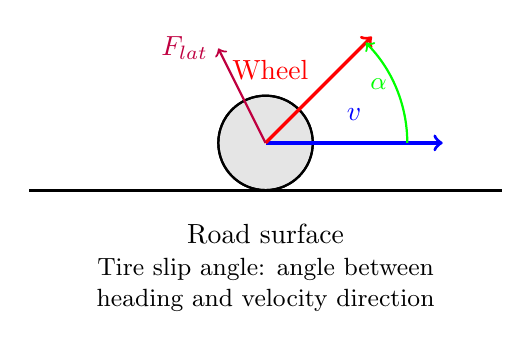
\begin{tikzpicture}[scale=1.5, thick]
    % Tire circle
    \draw[fill=black!10] (0, 0) circle (0.4);
    \draw[black] (0, 0) circle (0.4);

    % Contact patch (ground)
    \draw[very thick] (-2, -0.4) -- (2, -0.4);
    \node[below] at (0, -0.6) {Road surface};

    % Velocity vector (longitudinal)
    \draw[->, blue, very thick] (0, 0) -- (1.5, 0);
    \node[blue, above] at (0.75, 0.1) {$\vv{v}$};

    % Tire heading (rotated due to slip)
    \draw[->, red, very thick] (0, 0) -- (0.9, 0.9);
    \node[red, above left] at (0.45, 0.45) {Wheel};

    % Slip angle arc
    \draw[green, thick, ->] (1.2, 0) arc (0:45:1.2);
    \node[green, right, font=\small] at (0.8, 0.5) {$\alpha$};

    % Force vectors
    \draw[->, thick, purple] (0, 0) -- (-0.4, 0.8);
    \node[purple, left] at (-0.4, 0.8) {$F_{\text{lat}}$};

    % Labels
    \node[font=\small, align=center] at (0, -1.2) {Tire slip angle: angle between \\heading and velocity direction};
  \end{tikzpicture}
  \caption{Tire slip angle $\alpha$ is the angle between the tire's heading vector and its velocity direction. Lateral force $F_{\text{lat}}$ opposes the slip, creating steering effects.}
  \label{fig:slip-angle}
\end{figure}

% ==============================================================================
% DIAGRAM 3: WEIGHT TRANSFER
% ==============================================================================
% Use in Section 2 (Weight Transfer)

\begin{figure}[h]
  \centering
  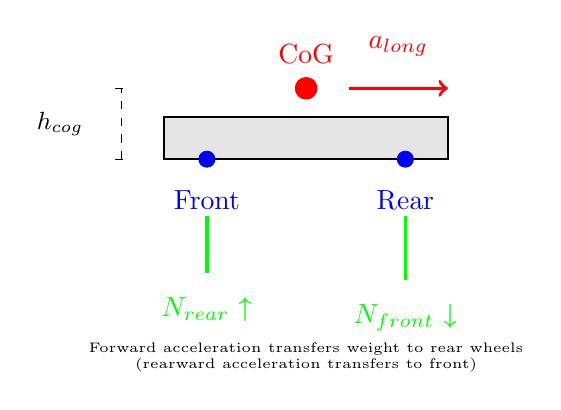
\begin{tikzpicture}[scale=1.8, thick]
    % Side view of car
    \draw[fill=gray!20] (-1, 0) rectangle (1, 0.3);
    \draw (-1, 0) -- (1, 0);

    % Wheel positions
    \fill[blue] (-0.7, 0) circle (0.06);
    \fill[blue] (0.7, 0) circle (0.06);
    \node[blue, below] at (-0.7, -0.15) {Front};
    \node[blue, below] at (0.7, -0.15) {Rear};

    % CoG
    \fill[red] (0, 0.5) circle (0.08);
    \node[red, above] at (0, 0.6) {CoG};

    % Height indication
    \draw[thin, dashed] (-1.3, 0) -- (-1.3, 0.5);
    \draw[thin, dashed] (-1.35, 0) -- (-1.25, 0);
    \draw[thin, dashed] (-1.35, 0.5) -- (-1.25, 0.5);
    \node[left, font=\small] at (-1.5, 0.25) {$h_{\text{cog}}$};

    % Acceleration arrow
    \draw[->, red, very thick] (0.3, 0.5) -- (1.0, 0.5);
    \node[red, above] at (0.65, 0.65) {$a_{\text{long}}$};

    % Weight transfer visualization
    \draw[green, very thick] (-0.7, -0.4) -- (-0.7, -0.8);
    \draw[green, very thick] (0.7, -0.4) -- (0.7, -0.85);
    \node[green, below] at (-0.7, -0.9) {$N_{\text{rear}}$ ↑};
    \node[green, below] at (0.7, -0.95) {$N_{\text{front}}$ ↓};

    \node[font=\tiny, align=center] at (0, -1.4) {Forward acceleration transfers weight to rear wheels \\ (rearward acceleration transfers to front)};
  \end{tikzpicture}
  \caption{Weight transfer during longitudinal acceleration: CoG height and acceleration magnitude determine the load shift between front and rear axles.}
  \label{fig:weight-transfer}
\end{figure}

% ==============================================================================
% DIAGRAM 4: FRICTION ELLIPSE (TRACTION CIRCLE)
% ==============================================================================
% Use in Section 5 (Tire Relaxation & Grip)

\begin{figure}[h]
  \centering
  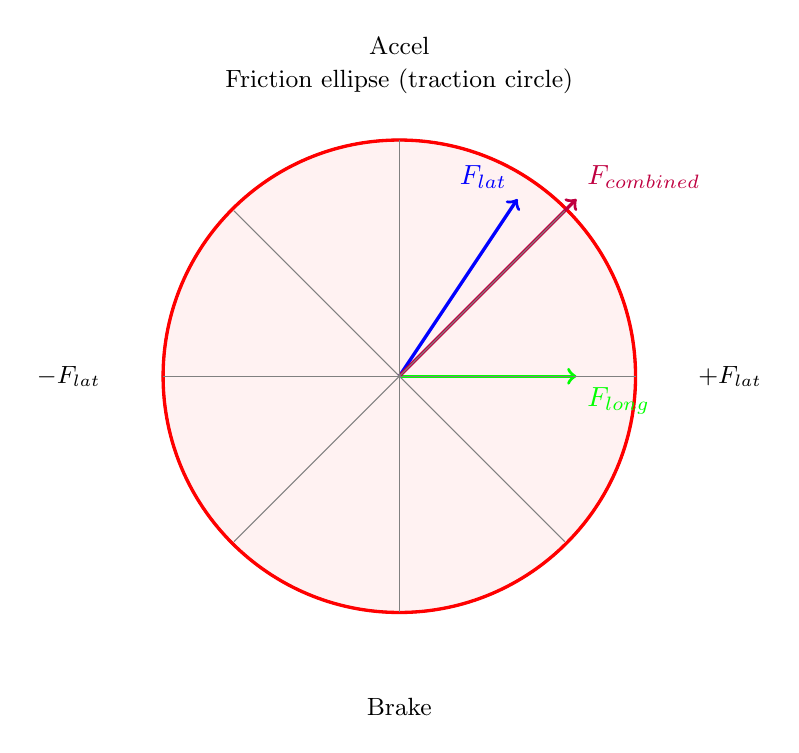
\begin{tikzpicture}[scale=1.5, thick]
    % Circle (friction limit)
    \draw[fill=red!5] (0, 0) circle (2);
    \draw[red, very thick] (0, 0) circle (2);

    % Force components
    \draw[->, blue, very thick] (0, 0) -- (1, 1.5) node[above left] {$F_{\text{lat}}$};
    \draw[->, green, very thick] (0, 0) -- (1.5, 0) node[below right] {$F_{\text{long}}$};
    \draw[->, purple, very thick] (0, 0) -- (1.5, 1.5) node[above right] {$F_{\text{combined}}$};

    % Grid
    \draw[thin, gray] (-2, 0) -- (2, 0);
    \draw[thin, gray] (0, -2) -- (0, 2);
    \draw[thin, gray] (-1.4, -1.4) -- (1.4, 1.4);
    \draw[thin, gray] (1.4, -1.4) -- (-1.4, 1.4);

    % Labels
    \node[font=\small] at (0, 2.5) {Friction ellipse (traction circle)};
    \node[font=\small] at (-2.8, 0) {$-F_{\text{lat}}$};
    \node[font=\small] at (2.8, 0) {$+F_{\text{lat}}$};
    \node[font=\small] at (0, -2.8) {Brake};
    \node[font=\small] at (0, 2.8) {Accel};
  \end{tikzpicture}
  \caption{Friction ellipse: Combined lateral and longitudinal forces cannot exceed the tire's grip circle $(N \cdot \mu)$. Exceeding the circle causes the tire to slip.}
  \label{fig:friction-ellipse}
\end{figure}

% ==============================================================================
% DIAGRAM 5: SELF-ALIGNING TORQUE (SAT)
% ==============================================================================
% Use in Section 6 (Steering & SAT)

\begin{figure}[h]
  \centering
  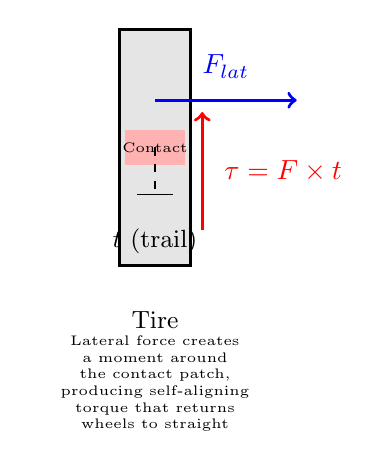
\begin{tikzpicture}[scale=1.5, thick]
    % Tire (top view)
    \draw[fill=gray!20] (-0.3, -1) rectangle (0.3, 1);
    \draw[black, very thick] (-0.3, -1) rectangle (0.3, 1);
    \node[font=\small, below] at (0, -1.3) {Tire};

    % Contact patch
    \fill[red!30] (-0.25, -0.15) rectangle (0.25, 0.15);
    \node[font=\tiny] at (0, 0) {Contact};

    % Lateral force
    \draw[->, blue, very thick] (0, 0.4) -- (1.2, 0.4);
    \node[blue, above] at (0.6, 0.5) {$F_{\text{lat}}$};

    % Pneumatic trail
    \draw[thin, dashed] (0, 0) -- (0, -0.4);
    \draw[thin] (-0.15, -0.4) -- (0.15, -0.4);
    \node[font=\small, below] at (0, -0.6) {$t$ (trail)};

    % Torque vector (out of page)
    \draw[->, red, very thick] (0.4, -0.7) -- (0.4, 0.3);
    \node[red, right] at (0.5, -0.2) {$\tau = F \times t$};

    % Explanation
    \node[font=\tiny, align=center, text width=3cm] at (0, -2) {Lateral force creates a moment around the contact patch, \\producing self-aligning torque that returns wheels to straight};
  \end{tikzpicture}
  \caption{Self-aligning torque (SAT): Product of lateral force and pneumatic trail creates a restoring torque that aligns tires with velocity direction.}
  \label{fig:sat}
\end{figure}

% ==============================================================================
% DIAGRAM 6: VERLET INTEGRATION CONCEPT
% ==============================================================================
% Use in Section 1 (Verlet Integration)

\begin{figure}[h]
  \centering
  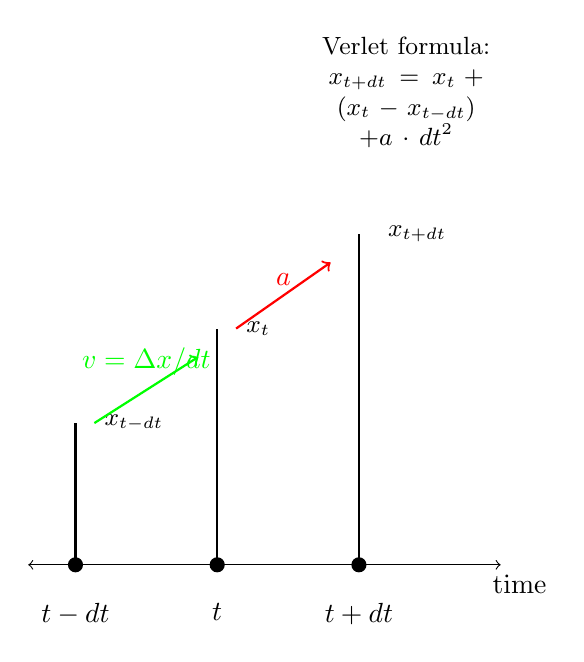
\begin{tikzpicture}[scale=1.2, thick]
    % Timeline
    \draw[<->, thin] (-0.5, 0) -- (4.5, 0);
    \node[below] at (4.7, 0) {time};

    % Time points
    \fill[black] (0, 0) circle (0.08);
    \fill[black] (1.5, 0) circle (0.08);
    \fill[black] (3, 0) circle (0.08);

    % Labels
    \node[below] at (0, -0.3) {$t - dt$};
    \node[below] at (1.5, -0.3) {$t$};
    \node[below] at (3, -0.3) {$t + dt$};

    % Positions on vertical axis
    \draw[thick] (0, 0) -- (0, 1.5);
    \draw[thick] (1.5, 0) -- (1.5, 2.5);
    \draw[thick] (3, 0) -- (3, 3.5);

    % Position labels
    \node[right, font=\small] at (0.2, 1.5) {$x_{t-dt}$};
    \node[right, font=\small] at (1.7, 2.5) {$x_t$};
    \node[right, font=\small] at (3.2, 3.5) {$x_{t+dt}$};

    % Velocity (implicit in position difference)
    \draw[->, green, thick] (0.2, 1.5) -- (1.3, 2.2);
    \node[green, above] at (0.75, 1.9) {$\vv{v} = \Delta x / dt$};

    % Acceleration
    \draw[->, red, thick] (1.7, 2.5) -- (2.7, 3.2);
    \node[red, above] at (2.2, 2.85) {$\vv{a}$};

    % Verlet formula
    \node[align=center, font=\small, text width=3cm] at (3.5, 5) {Verlet formula: \\
      $x_{t+dt} = x_t + (x_t - x_{t-dt})$ \\
      $+ \vv{a} \cdot dt^2$};
  \end{tikzpicture}
  \caption{Verlet integration: New position computed from previous position, velocity (implicit), and acceleration. Velocity is not explicitly stored.}
  \label{fig:verlet-concept}
\end{figure}

% ==============================================================================
% DIAGRAM 7: SPRING-DAMPER SYSTEM (CAMERA & STEERING)
% ==============================================================================
% Use in Section 8 (Camera & Rendering) or Section 6 (Steering)

\begin{figure}[h]
  \centering
  \begin{tikzpicture}[scale=1.5, thick]
    % Fixed support
    \draw[pattern=north west lines] (-2.5, 2) rectangle (-2, 1);
    \draw (-2.25, 2) -- (-2.25, 1);

    % Spring
    \draw (-2.25, 1.5) -- (-1.8, 1.3) -- (-1.5, 1.7) -- (-1.2, 1.3) -- (-0.9, 1.7) -- (-0.6, 1.3) -- (-0.3, 1.5);

    % Mass (box)
    \draw[fill=gray!40] (-0.3, 0.8) rectangle (0.3, 1.2);
    \draw[thick] (-0.3, 0.8) rectangle (0.3, 1.2);
    \node at (0, 1) {$m$};

    % Damper (piston)
    \draw[thick] (0.5, 0.8) -- (0.5, 1.2);
    \draw (0.3, 0.9) -- (0.5, 0.9);
    \draw (0.3, 1.1) -- (0.5, 1.1);

    % Fixed point for damper
    \draw[pattern=north west lines] (0.5, 0.6) rectangle (0.9, 0.8);

    % Labels
    \node[above] at (-1.5, 1.8) {Spring $k$};
    \node[above] at (0.7, 1.3) {Damper $c$};

    % Displacement
    \draw[<->, thin] (1.0, 0.5) -- (1.0, 1.5);
    \node[right] at (1.1, 1.0) {$x$};

    % Equation
    \node[align=center, font=\small, text width=3cm] at (0, -0.7) {Equation of motion: \\
      $m \ddot{x} = -kx - c\dot{x}$};
  \end{tikzpicture}
  \caption{Spring-damper system: Used for both camera following and steering column dynamics. Spring force $F_s = -kx$ and damping force $F_d = -c\dot{x}$.}
  \label{fig:spring-damper}
\end{figure}

% ==============================================================================
% DIAGRAM 8: GEAR RATIOS & TORQUE MULTIPLICATION
% ==============================================================================
% Use in Section 3 (Engine & Drivetrain)

\begin{figure}[h]
  \centering
  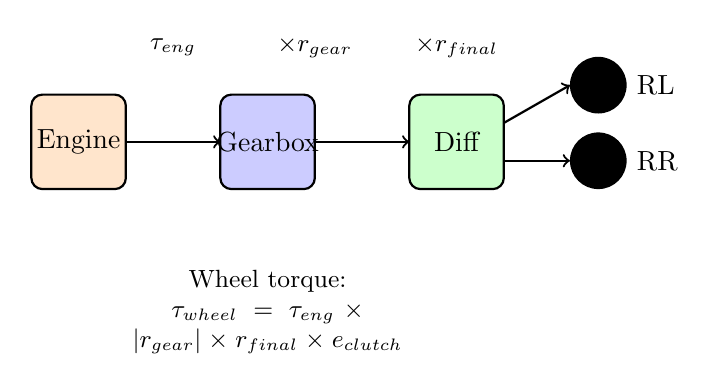
\begin{tikzpicture}[scale=1.2, thick]
    % Engine
    \draw[fill=orange!20, rounded corners] (-2.5, 0.3) rectangle (-1.5, 1.3);
    \node at (-2, 0.8) {Engine};

    % Gearbox
    \draw[fill=blue!20, rounded corners] (-0.5, 0.3) rectangle (0.5, 1.3);
    \node at (0, 0.8) {Gearbox};

    % Differential
    \draw[fill=green!20, rounded corners] (1.5, 0.3) rectangle (2.5, 1.3);
    \node at (2, 0.8) {Diff};

    % Wheels
    \fill[black] (3.5, 0.6) circle (0.3);
    \fill[black] (3.5, 1.4) circle (0.3);
    \node[right] at (3.8, 0.6) {RR};
    \node[right] at (3.8, 1.4) {RL};

    % Arrows
    \draw[->, thick] (-1.5, 0.8) -- (-0.5, 0.8);
    \draw[->, thick] (0.5, 0.8) -- (1.5, 0.8);
    \draw[->, thick] (2.5, 1.0) -- (3.2, 1.4);
    \draw[->, thick] (2.5, 0.6) -- (3.2, 0.6);

    % Ratios
    \node[font=\small] at (-1, 1.8) {$\tau_{\text{eng}}$};
    \node[font=\small] at (0.5, 1.8) {$\times r_{\text{gear}}$};
    \node[font=\small] at (2, 1.8) {$\times r_{\text{final}}$};

    % Formula
    \node[align=center, font=\small, text width=4cm] at (0, -1) {Wheel torque: \\
      $\tau_{\text{wheel}} = \tau_{\text{eng}} \times |r_{\text{gear}}| \times r_{\text{final}} \times e_{\text{clutch}}$};
  \end{tikzpicture}
  \caption{Drivetrain torque path: Engine torque is multiplied by gear ratio, final drive ratio, and clutch engagement factor before being applied to wheels.}
  \label{fig:drivetrain-path}
\end{figure}

% or individual diagrams can be copy-pasted where needed.

% ==============================================================================
% DIAGRAM 1: CAR BODY GEOMETRY
% ==============================================================================
% Use in Section 1 (Verlet Integration) to show car structure

\begin{figure}[h]
  \centering
  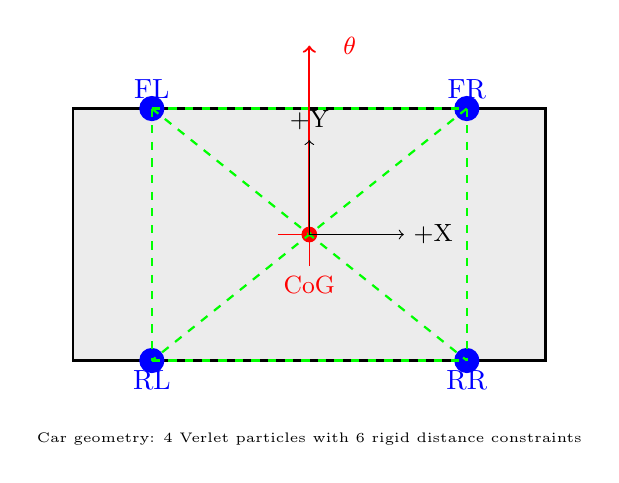
\begin{tikzpicture}[scale=2, thick]
    % Car body (rectangle)
    \draw[fill=lightgray!30] (-1.5, -0.8) rectangle (1.5, 0.8);
    \draw (-1.5, -0.8) -- (1.5, -0.8) -- (1.5, 0.8) -- (-1.5, 0.8) -- cycle;

    % Center of mass (crosshair)
    \fill[red] (0, 0) circle (0.05);
    \draw[red, thin] (-0.2, 0) -- (0.2, 0);
    \draw[red, thin] (0, -0.2) -- (0, 0.2);
    \node[red, below, font=\small] at (0, -0.2) {CoG};

    % Wheel positions (Verlet particles)
    \fill[blue] (-1.0, -0.8) circle (0.08);
    \fill[blue] (1.0, -0.8) circle (0.08);
    \fill[blue] (-1.0, 0.8) circle (0.08);
    \fill[blue] (1.0, 0.8) circle (0.08);

    % Labels
    \node[blue, above] at (-1.0, 0.8) {FL};
    \node[blue, above] at (1.0, 0.8) {FR};
    \node[blue, below] at (-1.0, -0.8) {RL};
    \node[blue, below] at (1.0, -0.8) {RR};

    % Constraints (dashed lines connecting particles)
    \draw[dashed, green] (-1.0, 0.8) -- (1.0, 0.8);  % Front axle
    \draw[dashed, green] (-1.0, -0.8) -- (1.0, -0.8); % Rear axle
    \draw[dashed, green] (-1.0, 0.8) -- (-1.0, -0.8); % Left side
    \draw[dashed, green] (1.0, 0.8) -- (1.0, -0.8);   % Right side
    \draw[dashed, green] (-1.0, 0.8) -- (1.0, -0.8);  % Diagonal
    \draw[dashed, green] (1.0, 0.8) -- (-1.0, -0.8);  % Diagonal

    % Heading vector
    \draw[->, red, thick] (0, 0) -- (0, 1.2);
    \node[red, right, font=\small] at (0.15, 1.2) {$\theta$};

    % Coordinate frame
    \draw[->, thin] (0, 0) -- (0.6, 0) node[right, font=\small] {+X};
    \draw[->, thin] (0, 0) -- (0, 0.6) node[above, font=\small] {+Y};

    \node[font=\tiny] at (0, -1.3) {Car geometry: 4 Verlet particles with 6 rigid distance constraints};
  \end{tikzpicture}
  \caption{VerletDrift car representation: Four wheel particles constrained to maintain rigid body shape. The center of gravity (CoG) is computed as average of front and rear midpoints.}
  \label{fig:car-geometry}
\end{figure}

% ==============================================================================
% DIAGRAM 2: TIRE SLIP ANGLE
% ==============================================================================
% Use in Section 4 (Tire Pacejka Model)

\begin{figure}[h]
  \centering
  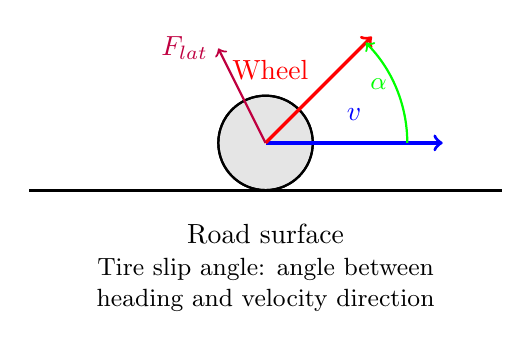
\begin{tikzpicture}[scale=1.5, thick]
    % Tire circle
    \draw[fill=black!10] (0, 0) circle (0.4);
    \draw[black] (0, 0) circle (0.4);

    % Contact patch (ground)
    \draw[very thick] (-2, -0.4) -- (2, -0.4);
    \node[below] at (0, -0.6) {Road surface};

    % Velocity vector (longitudinal)
    \draw[->, blue, very thick] (0, 0) -- (1.5, 0);
    \node[blue, above] at (0.75, 0.1) {$\vv{v}$};

    % Tire heading (rotated due to slip)
    \draw[->, red, very thick] (0, 0) -- (0.9, 0.9);
    \node[red, above left] at (0.45, 0.45) {Wheel};

    % Slip angle arc
    \draw[green, thick, ->] (1.2, 0) arc (0:45:1.2);
    \node[green, right, font=\small] at (0.8, 0.5) {$\alpha$};

    % Force vectors
    \draw[->, thick, purple] (0, 0) -- (-0.4, 0.8);
    \node[purple, left] at (-0.4, 0.8) {$F_{\text{lat}}$};

    % Labels
    \node[font=\small, align=center] at (0, -1.2) {Tire slip angle: angle between \\heading and velocity direction};
  \end{tikzpicture}
  \caption{Tire slip angle $\alpha$ is the angle between the tire's heading vector and its velocity direction. Lateral force $F_{\text{lat}}$ opposes the slip, creating steering effects.}
  \label{fig:slip-angle}
\end{figure}

% ==============================================================================
% DIAGRAM 3: WEIGHT TRANSFER
% ==============================================================================
% Use in Section 2 (Weight Transfer)

\begin{figure}[h]
  \centering
  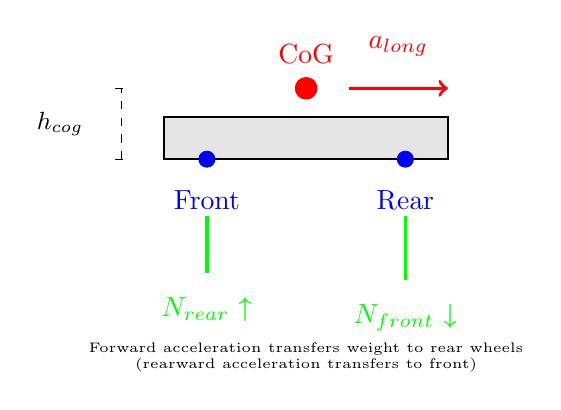
\begin{tikzpicture}[scale=1.8, thick]
    % Side view of car
    \draw[fill=gray!20] (-1, 0) rectangle (1, 0.3);
    \draw (-1, 0) -- (1, 0);

    % Wheel positions
    \fill[blue] (-0.7, 0) circle (0.06);
    \fill[blue] (0.7, 0) circle (0.06);
    \node[blue, below] at (-0.7, -0.15) {Front};
    \node[blue, below] at (0.7, -0.15) {Rear};

    % CoG
    \fill[red] (0, 0.5) circle (0.08);
    \node[red, above] at (0, 0.6) {CoG};

    % Height indication
    \draw[thin, dashed] (-1.3, 0) -- (-1.3, 0.5);
    \draw[thin, dashed] (-1.35, 0) -- (-1.25, 0);
    \draw[thin, dashed] (-1.35, 0.5) -- (-1.25, 0.5);
    \node[left, font=\small] at (-1.5, 0.25) {$h_{\text{cog}}$};

    % Acceleration arrow
    \draw[->, red, very thick] (0.3, 0.5) -- (1.0, 0.5);
    \node[red, above] at (0.65, 0.65) {$a_{\text{long}}$};

    % Weight transfer visualization
    \draw[green, very thick] (-0.7, -0.4) -- (-0.7, -0.8);
    \draw[green, very thick] (0.7, -0.4) -- (0.7, -0.85);
    \node[green, below] at (-0.7, -0.9) {$N_{\text{rear}}$ ↑};
    \node[green, below] at (0.7, -0.95) {$N_{\text{front}}$ ↓};

    \node[font=\tiny, align=center] at (0, -1.4) {Forward acceleration transfers weight to rear wheels \\ (rearward acceleration transfers to front)};
  \end{tikzpicture}
  \caption{Weight transfer during longitudinal acceleration: CoG height and acceleration magnitude determine the load shift between front and rear axles.}
  \label{fig:weight-transfer}
\end{figure}

% ==============================================================================
% DIAGRAM 4: FRICTION ELLIPSE (TRACTION CIRCLE)
% ==============================================================================
% Use in Section 5 (Tire Relaxation & Grip)

\begin{figure}[h]
  \centering
  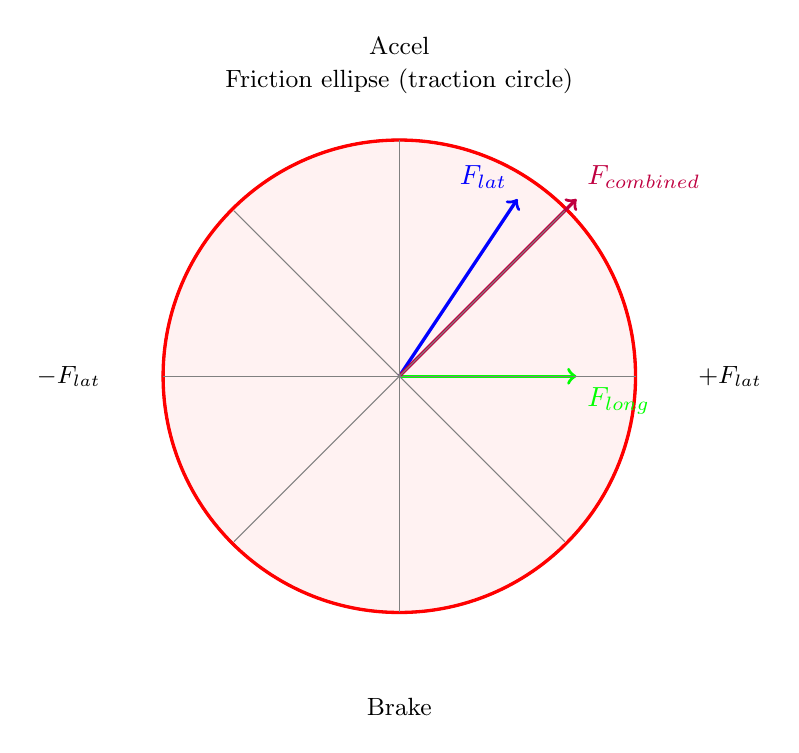
\begin{tikzpicture}[scale=1.5, thick]
    % Circle (friction limit)
    \draw[fill=red!5] (0, 0) circle (2);
    \draw[red, very thick] (0, 0) circle (2);

    % Force components
    \draw[->, blue, very thick] (0, 0) -- (1, 1.5) node[above left] {$F_{\text{lat}}$};
    \draw[->, green, very thick] (0, 0) -- (1.5, 0) node[below right] {$F_{\text{long}}$};
    \draw[->, purple, very thick] (0, 0) -- (1.5, 1.5) node[above right] {$F_{\text{combined}}$};

    % Grid
    \draw[thin, gray] (-2, 0) -- (2, 0);
    \draw[thin, gray] (0, -2) -- (0, 2);
    \draw[thin, gray] (-1.4, -1.4) -- (1.4, 1.4);
    \draw[thin, gray] (1.4, -1.4) -- (-1.4, 1.4);

    % Labels
    \node[font=\small] at (0, 2.5) {Friction ellipse (traction circle)};
    \node[font=\small] at (-2.8, 0) {$-F_{\text{lat}}$};
    \node[font=\small] at (2.8, 0) {$+F_{\text{lat}}$};
    \node[font=\small] at (0, -2.8) {Brake};
    \node[font=\small] at (0, 2.8) {Accel};
  \end{tikzpicture}
  \caption{Friction ellipse: Combined lateral and longitudinal forces cannot exceed the tire's grip circle $(N \cdot \mu)$. Exceeding the circle causes the tire to slip.}
  \label{fig:friction-ellipse}
\end{figure}

% ==============================================================================
% DIAGRAM 5: SELF-ALIGNING TORQUE (SAT)
% ==============================================================================
% Use in Section 6 (Steering & SAT)

\begin{figure}[h]
  \centering
  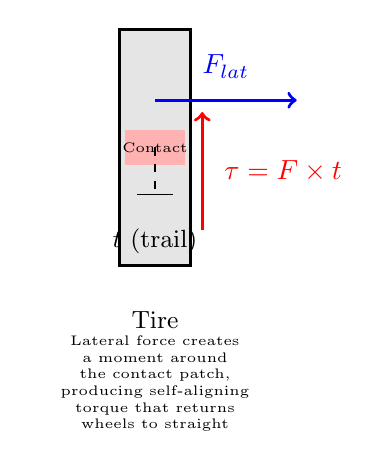
\begin{tikzpicture}[scale=1.5, thick]
    % Tire (top view)
    \draw[fill=gray!20] (-0.3, -1) rectangle (0.3, 1);
    \draw[black, very thick] (-0.3, -1) rectangle (0.3, 1);
    \node[font=\small, below] at (0, -1.3) {Tire};

    % Contact patch
    \fill[red!30] (-0.25, -0.15) rectangle (0.25, 0.15);
    \node[font=\tiny] at (0, 0) {Contact};

    % Lateral force
    \draw[->, blue, very thick] (0, 0.4) -- (1.2, 0.4);
    \node[blue, above] at (0.6, 0.5) {$F_{\text{lat}}$};

    % Pneumatic trail
    \draw[thin, dashed] (0, 0) -- (0, -0.4);
    \draw[thin] (-0.15, -0.4) -- (0.15, -0.4);
    \node[font=\small, below] at (0, -0.6) {$t$ (trail)};

    % Torque vector (out of page)
    \draw[->, red, very thick] (0.4, -0.7) -- (0.4, 0.3);
    \node[red, right] at (0.5, -0.2) {$\tau = F \times t$};

    % Explanation
    \node[font=\tiny, align=center, text width=3cm] at (0, -2) {Lateral force creates a moment around the contact patch, \\producing self-aligning torque that returns wheels to straight};
  \end{tikzpicture}
  \caption{Self-aligning torque (SAT): Product of lateral force and pneumatic trail creates a restoring torque that aligns tires with velocity direction.}
  \label{fig:sat}
\end{figure}

% ==============================================================================
% DIAGRAM 6: VERLET INTEGRATION CONCEPT
% ==============================================================================
% Use in Section 1 (Verlet Integration)

\begin{figure}[h]
  \centering
  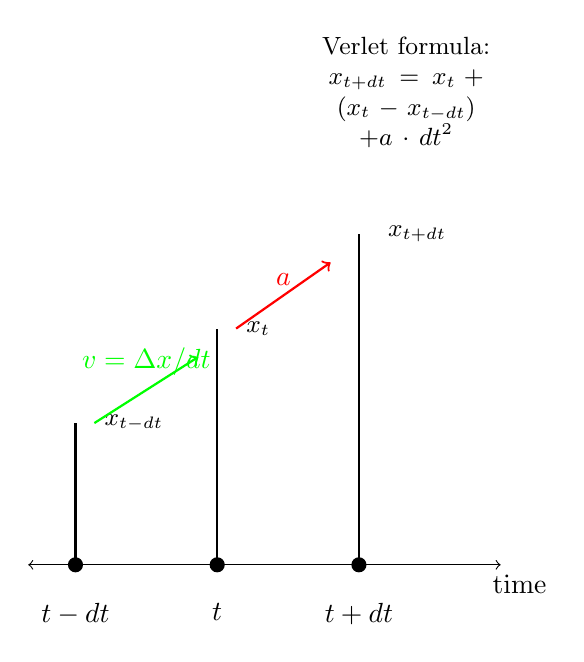
\begin{tikzpicture}[scale=1.2, thick]
    % Timeline
    \draw[<->, thin] (-0.5, 0) -- (4.5, 0);
    \node[below] at (4.7, 0) {time};

    % Time points
    \fill[black] (0, 0) circle (0.08);
    \fill[black] (1.5, 0) circle (0.08);
    \fill[black] (3, 0) circle (0.08);

    % Labels
    \node[below] at (0, -0.3) {$t - dt$};
    \node[below] at (1.5, -0.3) {$t$};
    \node[below] at (3, -0.3) {$t + dt$};

    % Positions on vertical axis
    \draw[thick] (0, 0) -- (0, 1.5);
    \draw[thick] (1.5, 0) -- (1.5, 2.5);
    \draw[thick] (3, 0) -- (3, 3.5);

    % Position labels
    \node[right, font=\small] at (0.2, 1.5) {$x_{t-dt}$};
    \node[right, font=\small] at (1.7, 2.5) {$x_t$};
    \node[right, font=\small] at (3.2, 3.5) {$x_{t+dt}$};

    % Velocity (implicit in position difference)
    \draw[->, green, thick] (0.2, 1.5) -- (1.3, 2.2);
    \node[green, above] at (0.75, 1.9) {$\vv{v} = \Delta x / dt$};

    % Acceleration
    \draw[->, red, thick] (1.7, 2.5) -- (2.7, 3.2);
    \node[red, above] at (2.2, 2.85) {$\vv{a}$};

    % Verlet formula
    \node[align=center, font=\small, text width=3cm] at (3.5, 5) {Verlet formula: \\
      $x_{t+dt} = x_t + (x_t - x_{t-dt})$ \\
      $+ \vv{a} \cdot dt^2$};
  \end{tikzpicture}
  \caption{Verlet integration: New position computed from previous position, velocity (implicit), and acceleration. Velocity is not explicitly stored.}
  \label{fig:verlet-concept}
\end{figure}

% ==============================================================================
% DIAGRAM 7: SPRING-DAMPER SYSTEM (CAMERA & STEERING)
% ==============================================================================
% Use in Section 8 (Camera & Rendering) or Section 6 (Steering)

\begin{figure}[h]
  \centering
  \begin{tikzpicture}[scale=1.5, thick]
    % Fixed support
    \draw[pattern=north west lines] (-2.5, 2) rectangle (-2, 1);
    \draw (-2.25, 2) -- (-2.25, 1);

    % Spring
    \draw (-2.25, 1.5) -- (-1.8, 1.3) -- (-1.5, 1.7) -- (-1.2, 1.3) -- (-0.9, 1.7) -- (-0.6, 1.3) -- (-0.3, 1.5);

    % Mass (box)
    \draw[fill=gray!40] (-0.3, 0.8) rectangle (0.3, 1.2);
    \draw[thick] (-0.3, 0.8) rectangle (0.3, 1.2);
    \node at (0, 1) {$m$};

    % Damper (piston)
    \draw[thick] (0.5, 0.8) -- (0.5, 1.2);
    \draw (0.3, 0.9) -- (0.5, 0.9);
    \draw (0.3, 1.1) -- (0.5, 1.1);

    % Fixed point for damper
    \draw[pattern=north west lines] (0.5, 0.6) rectangle (0.9, 0.8);

    % Labels
    \node[above] at (-1.5, 1.8) {Spring $k$};
    \node[above] at (0.7, 1.3) {Damper $c$};

    % Displacement
    \draw[<->, thin] (1.0, 0.5) -- (1.0, 1.5);
    \node[right] at (1.1, 1.0) {$x$};

    % Equation
    \node[align=center, font=\small, text width=3cm] at (0, -0.7) {Equation of motion: \\
      $m \ddot{x} = -kx - c\dot{x}$};
  \end{tikzpicture}
  \caption{Spring-damper system: Used for both camera following and steering column dynamics. Spring force $F_s = -kx$ and damping force $F_d = -c\dot{x}$.}
  \label{fig:spring-damper}
\end{figure}

% ==============================================================================
% DIAGRAM 8: GEAR RATIOS & TORQUE MULTIPLICATION
% ==============================================================================
% Use in Section 3 (Engine & Drivetrain)

\begin{figure}[h]
  \centering
  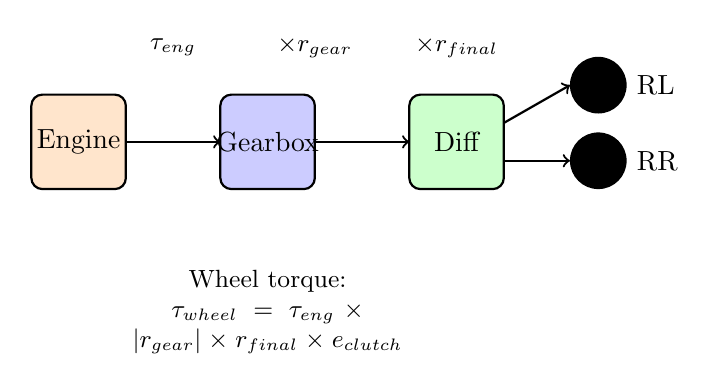
\begin{tikzpicture}[scale=1.2, thick]
    % Engine
    \draw[fill=orange!20, rounded corners] (-2.5, 0.3) rectangle (-1.5, 1.3);
    \node at (-2, 0.8) {Engine};

    % Gearbox
    \draw[fill=blue!20, rounded corners] (-0.5, 0.3) rectangle (0.5, 1.3);
    \node at (0, 0.8) {Gearbox};

    % Differential
    \draw[fill=green!20, rounded corners] (1.5, 0.3) rectangle (2.5, 1.3);
    \node at (2, 0.8) {Diff};

    % Wheels
    \fill[black] (3.5, 0.6) circle (0.3);
    \fill[black] (3.5, 1.4) circle (0.3);
    \node[right] at (3.8, 0.6) {RR};
    \node[right] at (3.8, 1.4) {RL};

    % Arrows
    \draw[->, thick] (-1.5, 0.8) -- (-0.5, 0.8);
    \draw[->, thick] (0.5, 0.8) -- (1.5, 0.8);
    \draw[->, thick] (2.5, 1.0) -- (3.2, 1.4);
    \draw[->, thick] (2.5, 0.6) -- (3.2, 0.6);

    % Ratios
    \node[font=\small] at (-1, 1.8) {$\tau_{\text{eng}}$};
    \node[font=\small] at (0.5, 1.8) {$\times r_{\text{gear}}$};
    \node[font=\small] at (2, 1.8) {$\times r_{\text{final}}$};

    % Formula
    \node[align=center, font=\small, text width=4cm] at (0, -1) {Wheel torque: \\
      $\tau_{\text{wheel}} = \tau_{\text{eng}} \times |r_{\text{gear}}| \times r_{\text{final}} \times e_{\text{clutch}}$};
  \end{tikzpicture}
  \caption{Drivetrain torque path: Engine torque is multiplied by gear ratio, final drive ratio, and clutch engagement factor before being applied to wheels.}
  \label{fig:drivetrain-path}
\end{figure}

% or individual diagrams can be copy-pasted where needed.

% ==============================================================================
% DIAGRAM 1: CAR BODY GEOMETRY
% ==============================================================================
% Use in Section 1 (Verlet Integration) to show car structure

\begin{figure}[h]
  \centering
  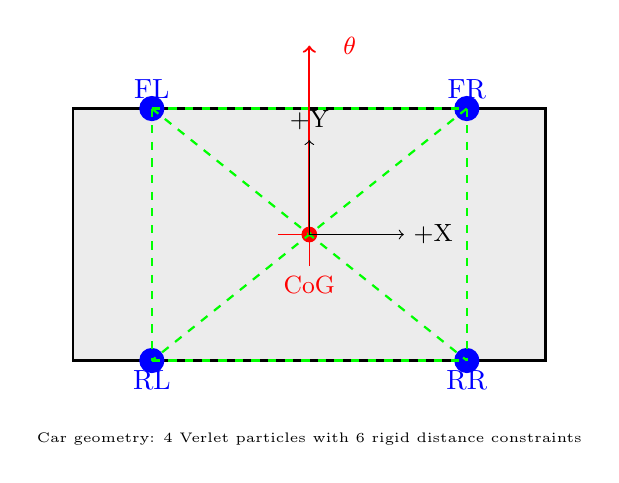
\begin{tikzpicture}[scale=2, thick]
    % Car body (rectangle)
    \draw[fill=lightgray!30] (-1.5, -0.8) rectangle (1.5, 0.8);
    \draw (-1.5, -0.8) -- (1.5, -0.8) -- (1.5, 0.8) -- (-1.5, 0.8) -- cycle;

    % Center of mass (crosshair)
    \fill[red] (0, 0) circle (0.05);
    \draw[red, thin] (-0.2, 0) -- (0.2, 0);
    \draw[red, thin] (0, -0.2) -- (0, 0.2);
    \node[red, below, font=\small] at (0, -0.2) {CoG};

    % Wheel positions (Verlet particles)
    \fill[blue] (-1.0, -0.8) circle (0.08);
    \fill[blue] (1.0, -0.8) circle (0.08);
    \fill[blue] (-1.0, 0.8) circle (0.08);
    \fill[blue] (1.0, 0.8) circle (0.08);

    % Labels
    \node[blue, above] at (-1.0, 0.8) {FL};
    \node[blue, above] at (1.0, 0.8) {FR};
    \node[blue, below] at (-1.0, -0.8) {RL};
    \node[blue, below] at (1.0, -0.8) {RR};

    % Constraints (dashed lines connecting particles)
    \draw[dashed, green] (-1.0, 0.8) -- (1.0, 0.8);  % Front axle
    \draw[dashed, green] (-1.0, -0.8) -- (1.0, -0.8); % Rear axle
    \draw[dashed, green] (-1.0, 0.8) -- (-1.0, -0.8); % Left side
    \draw[dashed, green] (1.0, 0.8) -- (1.0, -0.8);   % Right side
    \draw[dashed, green] (-1.0, 0.8) -- (1.0, -0.8);  % Diagonal
    \draw[dashed, green] (1.0, 0.8) -- (-1.0, -0.8);  % Diagonal

    % Heading vector
    \draw[->, red, thick] (0, 0) -- (0, 1.2);
    \node[red, right, font=\small] at (0.15, 1.2) {$\theta$};

    % Coordinate frame
    \draw[->, thin] (0, 0) -- (0.6, 0) node[right, font=\small] {+X};
    \draw[->, thin] (0, 0) -- (0, 0.6) node[above, font=\small] {+Y};

    \node[font=\tiny] at (0, -1.3) {Car geometry: 4 Verlet particles with 6 rigid distance constraints};
  \end{tikzpicture}
  \caption{VerletDrift car representation: Four wheel particles constrained to maintain rigid body shape. The center of gravity (CoG) is computed as average of front and rear midpoints.}
  \label{fig:car-geometry}
\end{figure}

% ==============================================================================
% DIAGRAM 2: TIRE SLIP ANGLE
% ==============================================================================
% Use in Section 4 (Tire Pacejka Model)

\begin{figure}[h]
  \centering
  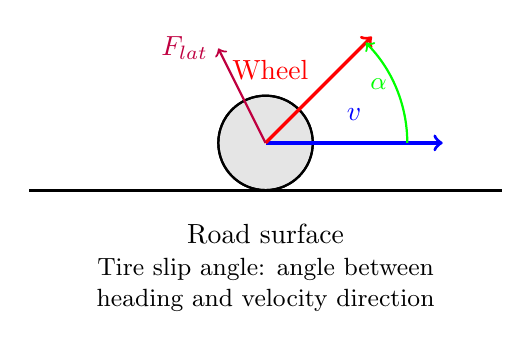
\begin{tikzpicture}[scale=1.5, thick]
    % Tire circle
    \draw[fill=black!10] (0, 0) circle (0.4);
    \draw[black] (0, 0) circle (0.4);

    % Contact patch (ground)
    \draw[very thick] (-2, -0.4) -- (2, -0.4);
    \node[below] at (0, -0.6) {Road surface};

    % Velocity vector (longitudinal)
    \draw[->, blue, very thick] (0, 0) -- (1.5, 0);
    \node[blue, above] at (0.75, 0.1) {$\vv{v}$};

    % Tire heading (rotated due to slip)
    \draw[->, red, very thick] (0, 0) -- (0.9, 0.9);
    \node[red, above left] at (0.45, 0.45) {Wheel};

    % Slip angle arc
    \draw[green, thick, ->] (1.2, 0) arc (0:45:1.2);
    \node[green, right, font=\small] at (0.8, 0.5) {$\alpha$};

    % Force vectors
    \draw[->, thick, purple] (0, 0) -- (-0.4, 0.8);
    \node[purple, left] at (-0.4, 0.8) {$F_{\text{lat}}$};

    % Labels
    \node[font=\small, align=center] at (0, -1.2) {Tire slip angle: angle between \\heading and velocity direction};
  \end{tikzpicture}
  \caption{Tire slip angle $\alpha$ is the angle between the tire's heading vector and its velocity direction. Lateral force $F_{\text{lat}}$ opposes the slip, creating steering effects.}
  \label{fig:slip-angle}
\end{figure}

% ==============================================================================
% DIAGRAM 3: WEIGHT TRANSFER
% ==============================================================================
% Use in Section 2 (Weight Transfer)

\begin{figure}[h]
  \centering
  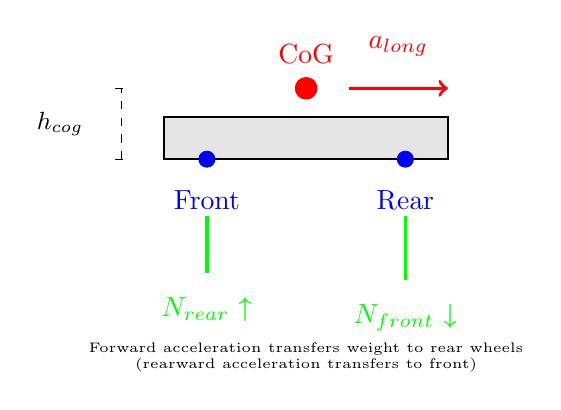
\begin{tikzpicture}[scale=1.8, thick]
    % Side view of car
    \draw[fill=gray!20] (-1, 0) rectangle (1, 0.3);
    \draw (-1, 0) -- (1, 0);

    % Wheel positions
    \fill[blue] (-0.7, 0) circle (0.06);
    \fill[blue] (0.7, 0) circle (0.06);
    \node[blue, below] at (-0.7, -0.15) {Front};
    \node[blue, below] at (0.7, -0.15) {Rear};

    % CoG
    \fill[red] (0, 0.5) circle (0.08);
    \node[red, above] at (0, 0.6) {CoG};

    % Height indication
    \draw[thin, dashed] (-1.3, 0) -- (-1.3, 0.5);
    \draw[thin, dashed] (-1.35, 0) -- (-1.25, 0);
    \draw[thin, dashed] (-1.35, 0.5) -- (-1.25, 0.5);
    \node[left, font=\small] at (-1.5, 0.25) {$h_{\text{cog}}$};

    % Acceleration arrow
    \draw[->, red, very thick] (0.3, 0.5) -- (1.0, 0.5);
    \node[red, above] at (0.65, 0.65) {$a_{\text{long}}$};

    % Weight transfer visualization
    \draw[green, very thick] (-0.7, -0.4) -- (-0.7, -0.8);
    \draw[green, very thick] (0.7, -0.4) -- (0.7, -0.85);
    \node[green, below] at (-0.7, -0.9) {$N_{\text{rear}}$ ↑};
    \node[green, below] at (0.7, -0.95) {$N_{\text{front}}$ ↓};

    \node[font=\tiny, align=center] at (0, -1.4) {Forward acceleration transfers weight to rear wheels \\ (rearward acceleration transfers to front)};
  \end{tikzpicture}
  \caption{Weight transfer during longitudinal acceleration: CoG height and acceleration magnitude determine the load shift between front and rear axles.}
  \label{fig:weight-transfer}
\end{figure}

% ==============================================================================
% DIAGRAM 4: FRICTION ELLIPSE (TRACTION CIRCLE)
% ==============================================================================
% Use in Section 5 (Tire Relaxation & Grip)

\begin{figure}[h]
  \centering
  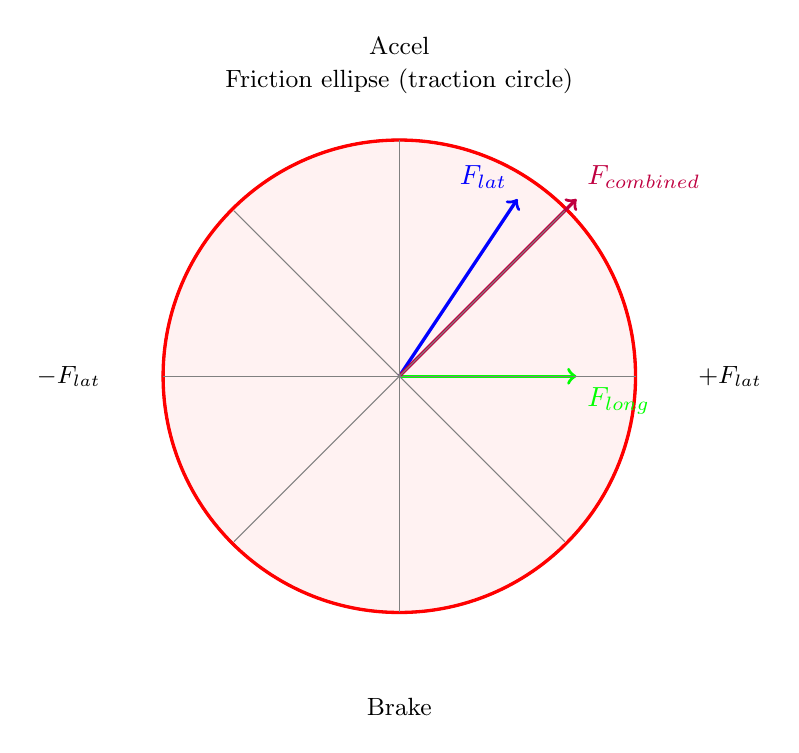
\begin{tikzpicture}[scale=1.5, thick]
    % Circle (friction limit)
    \draw[fill=red!5] (0, 0) circle (2);
    \draw[red, very thick] (0, 0) circle (2);

    % Force components
    \draw[->, blue, very thick] (0, 0) -- (1, 1.5) node[above left] {$F_{\text{lat}}$};
    \draw[->, green, very thick] (0, 0) -- (1.5, 0) node[below right] {$F_{\text{long}}$};
    \draw[->, purple, very thick] (0, 0) -- (1.5, 1.5) node[above right] {$F_{\text{combined}}$};

    % Grid
    \draw[thin, gray] (-2, 0) -- (2, 0);
    \draw[thin, gray] (0, -2) -- (0, 2);
    \draw[thin, gray] (-1.4, -1.4) -- (1.4, 1.4);
    \draw[thin, gray] (1.4, -1.4) -- (-1.4, 1.4);

    % Labels
    \node[font=\small] at (0, 2.5) {Friction ellipse (traction circle)};
    \node[font=\small] at (-2.8, 0) {$-F_{\text{lat}}$};
    \node[font=\small] at (2.8, 0) {$+F_{\text{lat}}$};
    \node[font=\small] at (0, -2.8) {Brake};
    \node[font=\small] at (0, 2.8) {Accel};
  \end{tikzpicture}
  \caption{Friction ellipse: Combined lateral and longitudinal forces cannot exceed the tire's grip circle $(N \cdot \mu)$. Exceeding the circle causes the tire to slip.}
  \label{fig:friction-ellipse}
\end{figure}

% ==============================================================================
% DIAGRAM 5: SELF-ALIGNING TORQUE (SAT)
% ==============================================================================
% Use in Section 6 (Steering & SAT)

\begin{figure}[h]
  \centering
  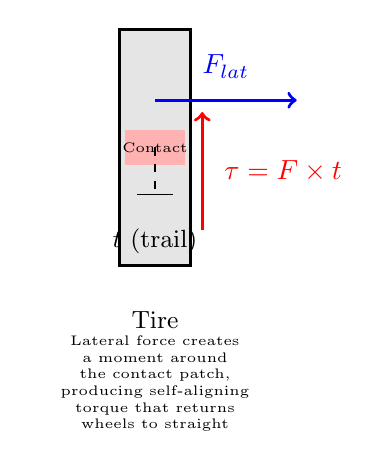
\begin{tikzpicture}[scale=1.5, thick]
    % Tire (top view)
    \draw[fill=gray!20] (-0.3, -1) rectangle (0.3, 1);
    \draw[black, very thick] (-0.3, -1) rectangle (0.3, 1);
    \node[font=\small, below] at (0, -1.3) {Tire};

    % Contact patch
    \fill[red!30] (-0.25, -0.15) rectangle (0.25, 0.15);
    \node[font=\tiny] at (0, 0) {Contact};

    % Lateral force
    \draw[->, blue, very thick] (0, 0.4) -- (1.2, 0.4);
    \node[blue, above] at (0.6, 0.5) {$F_{\text{lat}}$};

    % Pneumatic trail
    \draw[thin, dashed] (0, 0) -- (0, -0.4);
    \draw[thin] (-0.15, -0.4) -- (0.15, -0.4);
    \node[font=\small, below] at (0, -0.6) {$t$ (trail)};

    % Torque vector (out of page)
    \draw[->, red, very thick] (0.4, -0.7) -- (0.4, 0.3);
    \node[red, right] at (0.5, -0.2) {$\tau = F \times t$};

    % Explanation
    \node[font=\tiny, align=center, text width=3cm] at (0, -2) {Lateral force creates a moment around the contact patch, \\producing self-aligning torque that returns wheels to straight};
  \end{tikzpicture}
  \caption{Self-aligning torque (SAT): Product of lateral force and pneumatic trail creates a restoring torque that aligns tires with velocity direction.}
  \label{fig:sat}
\end{figure}

% ==============================================================================
% DIAGRAM 6: VERLET INTEGRATION CONCEPT
% ==============================================================================
% Use in Section 1 (Verlet Integration)

\begin{figure}[h]
  \centering
  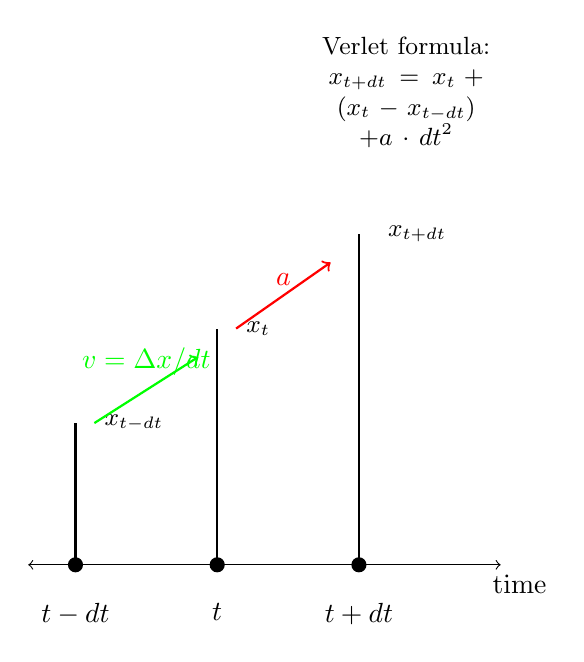
\begin{tikzpicture}[scale=1.2, thick]
    % Timeline
    \draw[<->, thin] (-0.5, 0) -- (4.5, 0);
    \node[below] at (4.7, 0) {time};

    % Time points
    \fill[black] (0, 0) circle (0.08);
    \fill[black] (1.5, 0) circle (0.08);
    \fill[black] (3, 0) circle (0.08);

    % Labels
    \node[below] at (0, -0.3) {$t - dt$};
    \node[below] at (1.5, -0.3) {$t$};
    \node[below] at (3, -0.3) {$t + dt$};

    % Positions on vertical axis
    \draw[thick] (0, 0) -- (0, 1.5);
    \draw[thick] (1.5, 0) -- (1.5, 2.5);
    \draw[thick] (3, 0) -- (3, 3.5);

    % Position labels
    \node[right, font=\small] at (0.2, 1.5) {$x_{t-dt}$};
    \node[right, font=\small] at (1.7, 2.5) {$x_t$};
    \node[right, font=\small] at (3.2, 3.5) {$x_{t+dt}$};

    % Velocity (implicit in position difference)
    \draw[->, green, thick] (0.2, 1.5) -- (1.3, 2.2);
    \node[green, above] at (0.75, 1.9) {$\vv{v} = \Delta x / dt$};

    % Acceleration
    \draw[->, red, thick] (1.7, 2.5) -- (2.7, 3.2);
    \node[red, above] at (2.2, 2.85) {$\vv{a}$};

    % Verlet formula
    \node[align=center, font=\small, text width=3cm] at (3.5, 5) {Verlet formula: \\
      $x_{t+dt} = x_t + (x_t - x_{t-dt})$ \\
      $+ \vv{a} \cdot dt^2$};
  \end{tikzpicture}
  \caption{Verlet integration: New position computed from previous position, velocity (implicit), and acceleration. Velocity is not explicitly stored.}
  \label{fig:verlet-concept}
\end{figure}

% ==============================================================================
% DIAGRAM 7: SPRING-DAMPER SYSTEM (CAMERA & STEERING)
% ==============================================================================
% Use in Section 8 (Camera & Rendering) or Section 6 (Steering)

\begin{figure}[h]
  \centering
  \begin{tikzpicture}[scale=1.5, thick]
    % Fixed support
    \draw[pattern=north west lines] (-2.5, 2) rectangle (-2, 1);
    \draw (-2.25, 2) -- (-2.25, 1);

    % Spring
    \draw (-2.25, 1.5) -- (-1.8, 1.3) -- (-1.5, 1.7) -- (-1.2, 1.3) -- (-0.9, 1.7) -- (-0.6, 1.3) -- (-0.3, 1.5);

    % Mass (box)
    \draw[fill=gray!40] (-0.3, 0.8) rectangle (0.3, 1.2);
    \draw[thick] (-0.3, 0.8) rectangle (0.3, 1.2);
    \node at (0, 1) {$m$};

    % Damper (piston)
    \draw[thick] (0.5, 0.8) -- (0.5, 1.2);
    \draw (0.3, 0.9) -- (0.5, 0.9);
    \draw (0.3, 1.1) -- (0.5, 1.1);

    % Fixed point for damper
    \draw[pattern=north west lines] (0.5, 0.6) rectangle (0.9, 0.8);

    % Labels
    \node[above] at (-1.5, 1.8) {Spring $k$};
    \node[above] at (0.7, 1.3) {Damper $c$};

    % Displacement
    \draw[<->, thin] (1.0, 0.5) -- (1.0, 1.5);
    \node[right] at (1.1, 1.0) {$x$};

    % Equation
    \node[align=center, font=\small, text width=3cm] at (0, -0.7) {Equation of motion: \\
      $m \ddot{x} = -kx - c\dot{x}$};
  \end{tikzpicture}
  \caption{Spring-damper system: Used for both camera following and steering column dynamics. Spring force $F_s = -kx$ and damping force $F_d = -c\dot{x}$.}
  \label{fig:spring-damper}
\end{figure}

% ==============================================================================
% DIAGRAM 8: GEAR RATIOS & TORQUE MULTIPLICATION
% ==============================================================================
% Use in Section 3 (Engine & Drivetrain)

\begin{figure}[h]
  \centering
  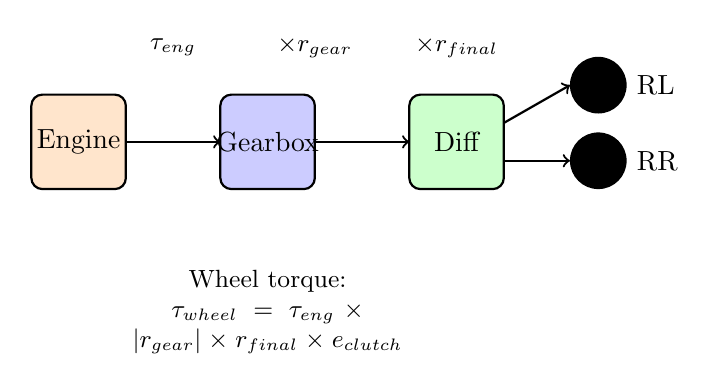
\begin{tikzpicture}[scale=1.2, thick]
    % Engine
    \draw[fill=orange!20, rounded corners] (-2.5, 0.3) rectangle (-1.5, 1.3);
    \node at (-2, 0.8) {Engine};

    % Gearbox
    \draw[fill=blue!20, rounded corners] (-0.5, 0.3) rectangle (0.5, 1.3);
    \node at (0, 0.8) {Gearbox};

    % Differential
    \draw[fill=green!20, rounded corners] (1.5, 0.3) rectangle (2.5, 1.3);
    \node at (2, 0.8) {Diff};

    % Wheels
    \fill[black] (3.5, 0.6) circle (0.3);
    \fill[black] (3.5, 1.4) circle (0.3);
    \node[right] at (3.8, 0.6) {RR};
    \node[right] at (3.8, 1.4) {RL};

    % Arrows
    \draw[->, thick] (-1.5, 0.8) -- (-0.5, 0.8);
    \draw[->, thick] (0.5, 0.8) -- (1.5, 0.8);
    \draw[->, thick] (2.5, 1.0) -- (3.2, 1.4);
    \draw[->, thick] (2.5, 0.6) -- (3.2, 0.6);

    % Ratios
    \node[font=\small] at (-1, 1.8) {$\tau_{\text{eng}}$};
    \node[font=\small] at (0.5, 1.8) {$\times r_{\text{gear}}$};
    \node[font=\small] at (2, 1.8) {$\times r_{\text{final}}$};

    % Formula
    \node[align=center, font=\small, text width=4cm] at (0, -1) {Wheel torque: \\
      $\tau_{\text{wheel}} = \tau_{\text{eng}} \times |r_{\text{gear}}| \times r_{\text{final}} \times e_{\text{clutch}}$};
  \end{tikzpicture}
  \caption{Drivetrain torque path: Engine torque is multiplied by gear ratio, final drive ratio, and clutch engagement factor before being applied to wheels.}
  \label{fig:drivetrain-path}
\end{figure}

% or individual diagrams can be copy-pasted where needed.

% ==============================================================================
% DIAGRAM 1: CAR BODY GEOMETRY
% ==============================================================================
% Use in Section 1 (Verlet Integration) to show car structure

\begin{figure}[h]
  \centering
  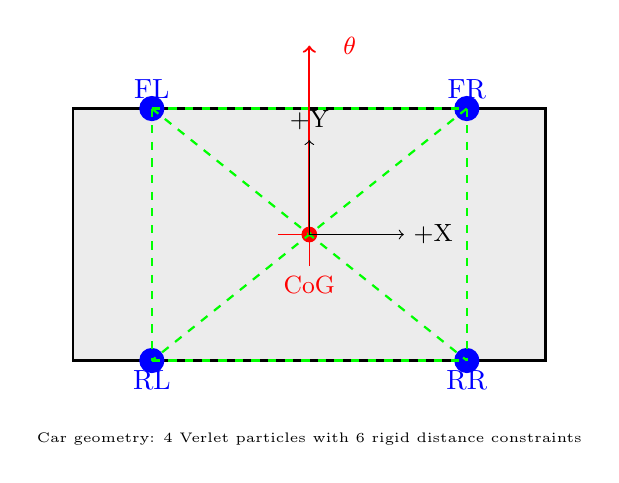
\begin{tikzpicture}[scale=2, thick]
    % Car body (rectangle)
    \draw[fill=lightgray!30] (-1.5, -0.8) rectangle (1.5, 0.8);
    \draw (-1.5, -0.8) -- (1.5, -0.8) -- (1.5, 0.8) -- (-1.5, 0.8) -- cycle;

    % Center of mass (crosshair)
    \fill[red] (0, 0) circle (0.05);
    \draw[red, thin] (-0.2, 0) -- (0.2, 0);
    \draw[red, thin] (0, -0.2) -- (0, 0.2);
    \node[red, below, font=\small] at (0, -0.2) {CoG};

    % Wheel positions (Verlet particles)
    \fill[blue] (-1.0, -0.8) circle (0.08);
    \fill[blue] (1.0, -0.8) circle (0.08);
    \fill[blue] (-1.0, 0.8) circle (0.08);
    \fill[blue] (1.0, 0.8) circle (0.08);

    % Labels
    \node[blue, above] at (-1.0, 0.8) {FL};
    \node[blue, above] at (1.0, 0.8) {FR};
    \node[blue, below] at (-1.0, -0.8) {RL};
    \node[blue, below] at (1.0, -0.8) {RR};

    % Constraints (dashed lines connecting particles)
    \draw[dashed, green] (-1.0, 0.8) -- (1.0, 0.8);  % Front axle
    \draw[dashed, green] (-1.0, -0.8) -- (1.0, -0.8); % Rear axle
    \draw[dashed, green] (-1.0, 0.8) -- (-1.0, -0.8); % Left side
    \draw[dashed, green] (1.0, 0.8) -- (1.0, -0.8);   % Right side
    \draw[dashed, green] (-1.0, 0.8) -- (1.0, -0.8);  % Diagonal
    \draw[dashed, green] (1.0, 0.8) -- (-1.0, -0.8);  % Diagonal

    % Heading vector
    \draw[->, red, thick] (0, 0) -- (0, 1.2);
    \node[red, right, font=\small] at (0.15, 1.2) {$\theta$};

    % Coordinate frame
    \draw[->, thin] (0, 0) -- (0.6, 0) node[right, font=\small] {+X};
    \draw[->, thin] (0, 0) -- (0, 0.6) node[above, font=\small] {+Y};

    \node[font=\tiny] at (0, -1.3) {Car geometry: 4 Verlet particles with 6 rigid distance constraints};
  \end{tikzpicture}
  \caption{VerletDrift car representation: Four wheel particles constrained to maintain rigid body shape. The center of gravity (CoG) is computed as average of front and rear midpoints.}
  \label{fig:car-geometry}
\end{figure}

% ==============================================================================
% DIAGRAM 2: TIRE SLIP ANGLE
% ==============================================================================
% Use in Section 4 (Tire Pacejka Model)

\begin{figure}[h]
  \centering
  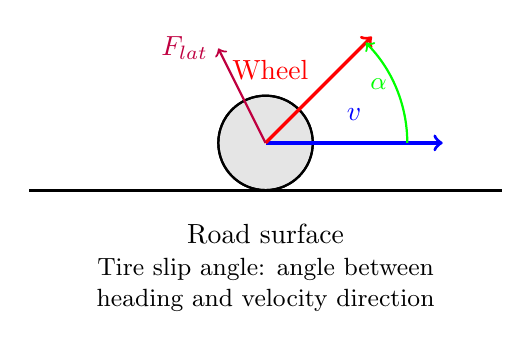
\begin{tikzpicture}[scale=1.5, thick]
    % Tire circle
    \draw[fill=black!10] (0, 0) circle (0.4);
    \draw[black] (0, 0) circle (0.4);

    % Contact patch (ground)
    \draw[very thick] (-2, -0.4) -- (2, -0.4);
    \node[below] at (0, -0.6) {Road surface};

    % Velocity vector (longitudinal)
    \draw[->, blue, very thick] (0, 0) -- (1.5, 0);
    \node[blue, above] at (0.75, 0.1) {$\vv{v}$};

    % Tire heading (rotated due to slip)
    \draw[->, red, very thick] (0, 0) -- (0.9, 0.9);
    \node[red, above left] at (0.45, 0.45) {Wheel};

    % Slip angle arc
    \draw[green, thick, ->] (1.2, 0) arc (0:45:1.2);
    \node[green, right, font=\small] at (0.8, 0.5) {$\alpha$};

    % Force vectors
    \draw[->, thick, purple] (0, 0) -- (-0.4, 0.8);
    \node[purple, left] at (-0.4, 0.8) {$F_{\text{lat}}$};

    % Labels
    \node[font=\small, align=center] at (0, -1.2) {Tire slip angle: angle between \\heading and velocity direction};
  \end{tikzpicture}
  \caption{Tire slip angle $\alpha$ is the angle between the tire's heading vector and its velocity direction. Lateral force $F_{\text{lat}}$ opposes the slip, creating steering effects.}
  \label{fig:slip-angle}
\end{figure}

% ==============================================================================
% DIAGRAM 3: WEIGHT TRANSFER
% ==============================================================================
% Use in Section 2 (Weight Transfer)

\begin{figure}[h]
  \centering
  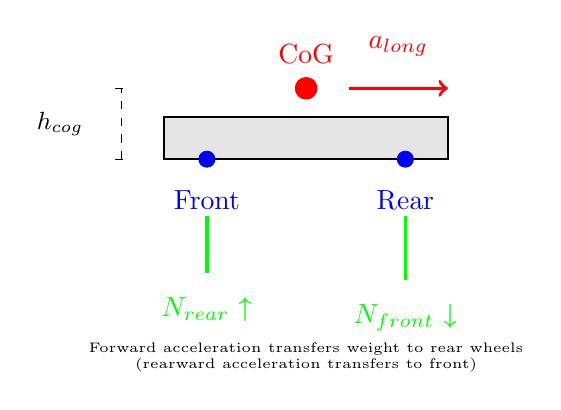
\begin{tikzpicture}[scale=1.8, thick]
    % Side view of car
    \draw[fill=gray!20] (-1, 0) rectangle (1, 0.3);
    \draw (-1, 0) -- (1, 0);

    % Wheel positions
    \fill[blue] (-0.7, 0) circle (0.06);
    \fill[blue] (0.7, 0) circle (0.06);
    \node[blue, below] at (-0.7, -0.15) {Front};
    \node[blue, below] at (0.7, -0.15) {Rear};

    % CoG
    \fill[red] (0, 0.5) circle (0.08);
    \node[red, above] at (0, 0.6) {CoG};

    % Height indication
    \draw[thin, dashed] (-1.3, 0) -- (-1.3, 0.5);
    \draw[thin, dashed] (-1.35, 0) -- (-1.25, 0);
    \draw[thin, dashed] (-1.35, 0.5) -- (-1.25, 0.5);
    \node[left, font=\small] at (-1.5, 0.25) {$h_{\text{cog}}$};

    % Acceleration arrow
    \draw[->, red, very thick] (0.3, 0.5) -- (1.0, 0.5);
    \node[red, above] at (0.65, 0.65) {$a_{\text{long}}$};

    % Weight transfer visualization
    \draw[green, very thick] (-0.7, -0.4) -- (-0.7, -0.8);
    \draw[green, very thick] (0.7, -0.4) -- (0.7, -0.85);
    \node[green, below] at (-0.7, -0.9) {$N_{\text{rear}}$ ↑};
    \node[green, below] at (0.7, -0.95) {$N_{\text{front}}$ ↓};

    \node[font=\tiny, align=center] at (0, -1.4) {Forward acceleration transfers weight to rear wheels \\ (rearward acceleration transfers to front)};
  \end{tikzpicture}
  \caption{Weight transfer during longitudinal acceleration: CoG height and acceleration magnitude determine the load shift between front and rear axles.}
  \label{fig:weight-transfer}
\end{figure}

% ==============================================================================
% DIAGRAM 4: FRICTION ELLIPSE (TRACTION CIRCLE)
% ==============================================================================
% Use in Section 5 (Tire Relaxation & Grip)

\begin{figure}[h]
  \centering
  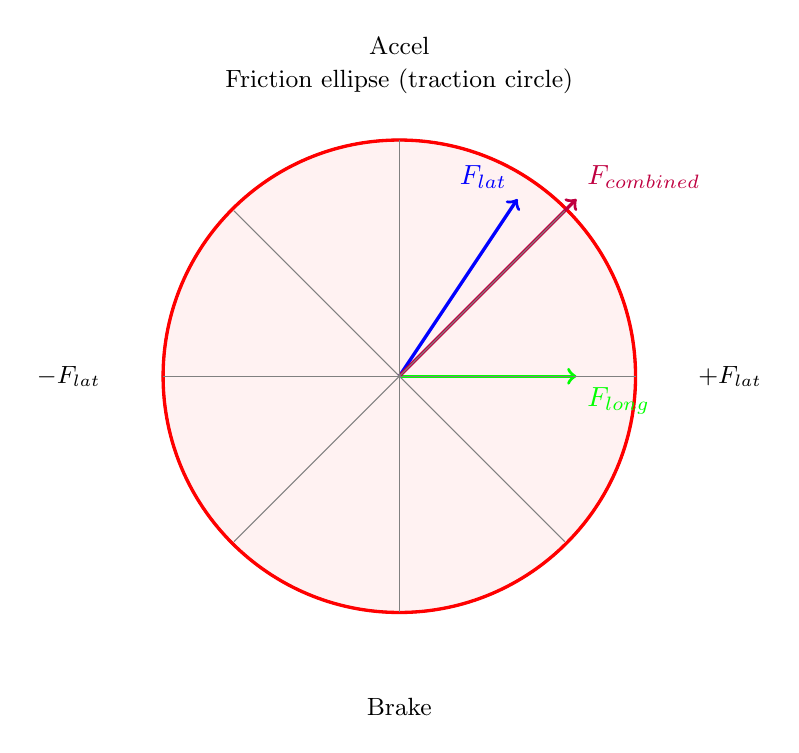
\begin{tikzpicture}[scale=1.5, thick]
    % Circle (friction limit)
    \draw[fill=red!5] (0, 0) circle (2);
    \draw[red, very thick] (0, 0) circle (2);

    % Force components
    \draw[->, blue, very thick] (0, 0) -- (1, 1.5) node[above left] {$F_{\text{lat}}$};
    \draw[->, green, very thick] (0, 0) -- (1.5, 0) node[below right] {$F_{\text{long}}$};
    \draw[->, purple, very thick] (0, 0) -- (1.5, 1.5) node[above right] {$F_{\text{combined}}$};

    % Grid
    \draw[thin, gray] (-2, 0) -- (2, 0);
    \draw[thin, gray] (0, -2) -- (0, 2);
    \draw[thin, gray] (-1.4, -1.4) -- (1.4, 1.4);
    \draw[thin, gray] (1.4, -1.4) -- (-1.4, 1.4);

    % Labels
    \node[font=\small] at (0, 2.5) {Friction ellipse (traction circle)};
    \node[font=\small] at (-2.8, 0) {$-F_{\text{lat}}$};
    \node[font=\small] at (2.8, 0) {$+F_{\text{lat}}$};
    \node[font=\small] at (0, -2.8) {Brake};
    \node[font=\small] at (0, 2.8) {Accel};
  \end{tikzpicture}
  \caption{Friction ellipse: Combined lateral and longitudinal forces cannot exceed the tire's grip circle $(N \cdot \mu)$. Exceeding the circle causes the tire to slip.}
  \label{fig:friction-ellipse}
\end{figure}

% ==============================================================================
% DIAGRAM 5: SELF-ALIGNING TORQUE (SAT)
% ==============================================================================
% Use in Section 6 (Steering & SAT)

\begin{figure}[h]
  \centering
  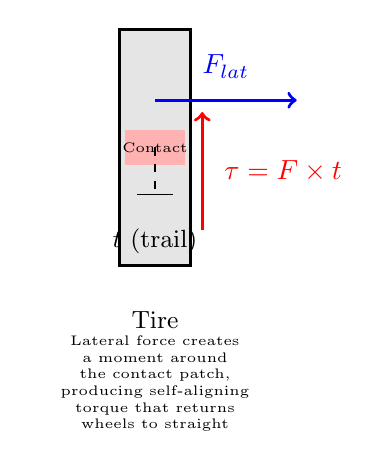
\begin{tikzpicture}[scale=1.5, thick]
    % Tire (top view)
    \draw[fill=gray!20] (-0.3, -1) rectangle (0.3, 1);
    \draw[black, very thick] (-0.3, -1) rectangle (0.3, 1);
    \node[font=\small, below] at (0, -1.3) {Tire};

    % Contact patch
    \fill[red!30] (-0.25, -0.15) rectangle (0.25, 0.15);
    \node[font=\tiny] at (0, 0) {Contact};

    % Lateral force
    \draw[->, blue, very thick] (0, 0.4) -- (1.2, 0.4);
    \node[blue, above] at (0.6, 0.5) {$F_{\text{lat}}$};

    % Pneumatic trail
    \draw[thin, dashed] (0, 0) -- (0, -0.4);
    \draw[thin] (-0.15, -0.4) -- (0.15, -0.4);
    \node[font=\small, below] at (0, -0.6) {$t$ (trail)};

    % Torque vector (out of page)
    \draw[->, red, very thick] (0.4, -0.7) -- (0.4, 0.3);
    \node[red, right] at (0.5, -0.2) {$\tau = F \times t$};

    % Explanation
    \node[font=\tiny, align=center, text width=3cm] at (0, -2) {Lateral force creates a moment around the contact patch, \\producing self-aligning torque that returns wheels to straight};
  \end{tikzpicture}
  \caption{Self-aligning torque (SAT): Product of lateral force and pneumatic trail creates a restoring torque that aligns tires with velocity direction.}
  \label{fig:sat}
\end{figure}

% ==============================================================================
% DIAGRAM 6: VERLET INTEGRATION CONCEPT
% ==============================================================================
% Use in Section 1 (Verlet Integration)

\begin{figure}[h]
  \centering
  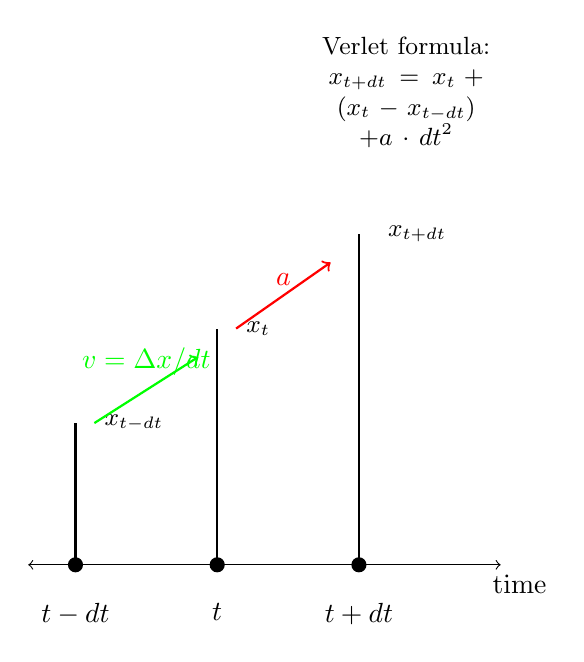
\begin{tikzpicture}[scale=1.2, thick]
    % Timeline
    \draw[<->, thin] (-0.5, 0) -- (4.5, 0);
    \node[below] at (4.7, 0) {time};

    % Time points
    \fill[black] (0, 0) circle (0.08);
    \fill[black] (1.5, 0) circle (0.08);
    \fill[black] (3, 0) circle (0.08);

    % Labels
    \node[below] at (0, -0.3) {$t - dt$};
    \node[below] at (1.5, -0.3) {$t$};
    \node[below] at (3, -0.3) {$t + dt$};

    % Positions on vertical axis
    \draw[thick] (0, 0) -- (0, 1.5);
    \draw[thick] (1.5, 0) -- (1.5, 2.5);
    \draw[thick] (3, 0) -- (3, 3.5);

    % Position labels
    \node[right, font=\small] at (0.2, 1.5) {$x_{t-dt}$};
    \node[right, font=\small] at (1.7, 2.5) {$x_t$};
    \node[right, font=\small] at (3.2, 3.5) {$x_{t+dt}$};

    % Velocity (implicit in position difference)
    \draw[->, green, thick] (0.2, 1.5) -- (1.3, 2.2);
    \node[green, above] at (0.75, 1.9) {$\vv{v} = \Delta x / dt$};

    % Acceleration
    \draw[->, red, thick] (1.7, 2.5) -- (2.7, 3.2);
    \node[red, above] at (2.2, 2.85) {$\vv{a}$};

    % Verlet formula
    \node[align=center, font=\small, text width=3cm] at (3.5, 5) {Verlet formula: \\
      $x_{t+dt} = x_t + (x_t - x_{t-dt})$ \\
      $+ \vv{a} \cdot dt^2$};
  \end{tikzpicture}
  \caption{Verlet integration: New position computed from previous position, velocity (implicit), and acceleration. Velocity is not explicitly stored.}
  \label{fig:verlet-concept}
\end{figure}

% ==============================================================================
% DIAGRAM 7: SPRING-DAMPER SYSTEM (CAMERA & STEERING)
% ==============================================================================
% Use in Section 8 (Camera & Rendering) or Section 6 (Steering)

\begin{figure}[h]
  \centering
  \begin{tikzpicture}[scale=1.5, thick]
    % Fixed support
    \draw[pattern=north west lines] (-2.5, 2) rectangle (-2, 1);
    \draw (-2.25, 2) -- (-2.25, 1);

    % Spring
    \draw (-2.25, 1.5) -- (-1.8, 1.3) -- (-1.5, 1.7) -- (-1.2, 1.3) -- (-0.9, 1.7) -- (-0.6, 1.3) -- (-0.3, 1.5);

    % Mass (box)
    \draw[fill=gray!40] (-0.3, 0.8) rectangle (0.3, 1.2);
    \draw[thick] (-0.3, 0.8) rectangle (0.3, 1.2);
    \node at (0, 1) {$m$};

    % Damper (piston)
    \draw[thick] (0.5, 0.8) -- (0.5, 1.2);
    \draw (0.3, 0.9) -- (0.5, 0.9);
    \draw (0.3, 1.1) -- (0.5, 1.1);

    % Fixed point for damper
    \draw[pattern=north west lines] (0.5, 0.6) rectangle (0.9, 0.8);

    % Labels
    \node[above] at (-1.5, 1.8) {Spring $k$};
    \node[above] at (0.7, 1.3) {Damper $c$};

    % Displacement
    \draw[<->, thin] (1.0, 0.5) -- (1.0, 1.5);
    \node[right] at (1.1, 1.0) {$x$};

    % Equation
    \node[align=center, font=\small, text width=3cm] at (0, -0.7) {Equation of motion: \\
      $m \ddot{x} = -kx - c\dot{x}$};
  \end{tikzpicture}
  \caption{Spring-damper system: Used for both camera following and steering column dynamics. Spring force $F_s = -kx$ and damping force $F_d = -c\dot{x}$.}
  \label{fig:spring-damper}
\end{figure}

% ==============================================================================
% DIAGRAM 8: GEAR RATIOS & TORQUE MULTIPLICATION
% ==============================================================================
% Use in Section 3 (Engine & Drivetrain)

\begin{figure}[h]
  \centering
  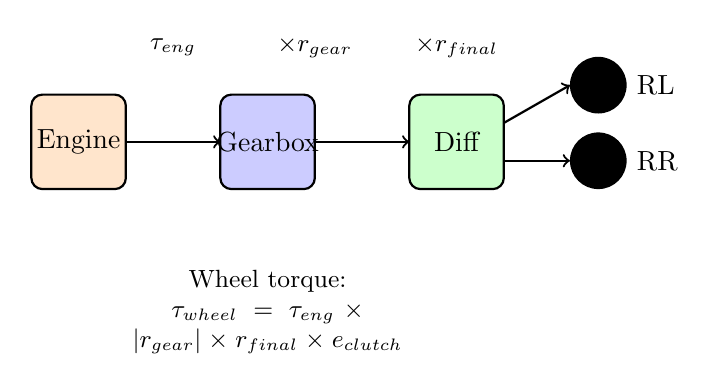
\begin{tikzpicture}[scale=1.2, thick]
    % Engine
    \draw[fill=orange!20, rounded corners] (-2.5, 0.3) rectangle (-1.5, 1.3);
    \node at (-2, 0.8) {Engine};

    % Gearbox
    \draw[fill=blue!20, rounded corners] (-0.5, 0.3) rectangle (0.5, 1.3);
    \node at (0, 0.8) {Gearbox};

    % Differential
    \draw[fill=green!20, rounded corners] (1.5, 0.3) rectangle (2.5, 1.3);
    \node at (2, 0.8) {Diff};

    % Wheels
    \fill[black] (3.5, 0.6) circle (0.3);
    \fill[black] (3.5, 1.4) circle (0.3);
    \node[right] at (3.8, 0.6) {RR};
    \node[right] at (3.8, 1.4) {RL};

    % Arrows
    \draw[->, thick] (-1.5, 0.8) -- (-0.5, 0.8);
    \draw[->, thick] (0.5, 0.8) -- (1.5, 0.8);
    \draw[->, thick] (2.5, 1.0) -- (3.2, 1.4);
    \draw[->, thick] (2.5, 0.6) -- (3.2, 0.6);

    % Ratios
    \node[font=\small] at (-1, 1.8) {$\tau_{\text{eng}}$};
    \node[font=\small] at (0.5, 1.8) {$\times r_{\text{gear}}$};
    \node[font=\small] at (2, 1.8) {$\times r_{\text{final}}$};

    % Formula
    \node[align=center, font=\small, text width=4cm] at (0, -1) {Wheel torque: \\
      $\tau_{\text{wheel}} = \tau_{\text{eng}} \times |r_{\text{gear}}| \times r_{\text{final}} \times e_{\text{clutch}}$};
  \end{tikzpicture}
  \caption{Drivetrain torque path: Engine torque is multiplied by gear ratio, final drive ratio, and clutch engagement factor before being applied to wheels.}
  \label{fig:drivetrain-path}
\end{figure}
